\section{二维码结构和编码}
二维码可以分为行排式(堆叠式)二维码和矩阵式二维码。\\
行排式/堆叠式二维码形态上是由多行短截的一维条码堆叠而成。
行排式/堆叠式二维码的编码原理是建立在一维条码基础之上的,按需要堆积成多行。它在编码设计、校验原理、识读方式等方面继承了一维条码的一些特点,识读设备与条码印刷和一维条码技术兼容。
代表性的行排式二维码有Code49,Code 16k,PDF417等。\\
矩阵式二维码以矩阵的形式组成,在矩阵相应元素位置上用“点”表示二进制的“1”,用“空”表示二进制的“0”,有“点”和“空”的排列组成信息编码。
矩阵式二维码是一种原理和方法与行排式二维码完全不同的条码系统。
行排式二维码和一维条码的编码都是对条码黑白相间条空的宽度进行调制,而矩阵码是对条码整个编码区域内的点进行编码,所以矩阵码有比行排式二维码高得多的信息密度。
行排式二维码只是在形式上像二维码,而本质上完全属于一维条码,所以有人也称行排式二维码为1.5维条码,而矩阵码才是真正的二维条码。
代表性的矩阵式二维码有QR Code,Code One,Data Matrix等。\\
由于QR码在日常生活中应用最为广泛,本篇报告着重研究QR码的检测。

\subsection{QR码的结构}
QR码由正方形方格组成,组成正方形阵列。
它由编码区域和包括定位模块,分隔线,修正模块,对齐模块在内的功能图形组成。
功能图形不能用于数据编码。
符号的四周由空白区域包围。
QR码的编码示意如图\ref{fig:structure1}。

\begin{figure}[h]
\centering
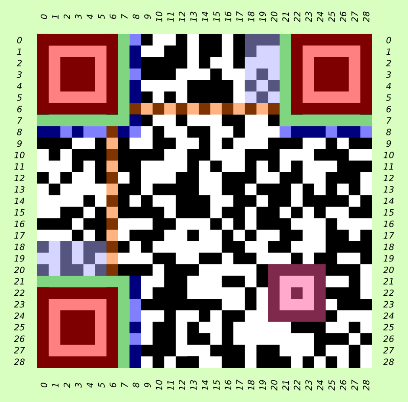
\includegraphics[width=0.9\linewidth]{structure1}
\caption[QR码结构]{QR码结构}
\label{fig:structure1}
\end{figure}

QR码的最小组成单元是方格,白色代表二进制“0”,黑色代表二进制“1”,如图\ref{fig:structure2}定义。

\begin{figure}[h]
\centering
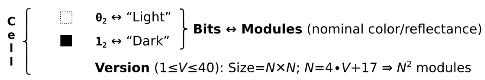
\includegraphics[width=0.9\linewidth]{structure2}
\caption[cell]{QR码的最小单元}
\label{fig:structure2}
\end{figure}

图\ref{fig:structure1}中的功能图形分为分隔线,定位模块,对齐模块,修正模块等,如图\ref{fig:structure3}所示。

\begin{figure}[h]
\centering
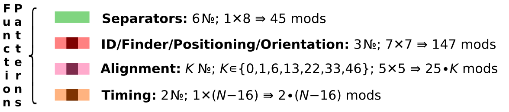
\includegraphics[width=0.9\linewidth]{structure3}
\caption[functional]{QR码的功能图形}
\label{fig:structure3}
\end{figure}

图\ref{fig:structure1}中的编码区域分为格式信息,版本信息和数据内容,如图\ref{fig:structure4}所示。

\begin{figure}[h]
\centering
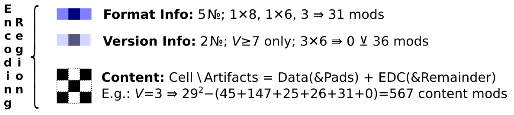
\includegraphics[width=0.9\linewidth]{structure4}
\caption[content]{QR码的编码区域}
\label{fig:structure4}
\end{figure}

各个模块的具体说明如下:\\ \\
(1).符号版本和规格\\
QR码符号共有40种规格,分别是版本1~版本40。版本1的规格为21*21个方格,版本2的规格为25*25个方格。以此类推,版本N的规格为$ (21+4*(N-1))^2 $个方格。\\
(2).定位模块\\
定位模块包括3个位置相同的位置探测图形,分别位于二维码图形的左上角、右上角和左下角。每个位置探测图形可以看作是由3个重叠的同心正方形组成,分别为7*7个黑色方格、5*5个白色方格,3*3个黑色方格。位置探测图形的模块宽度比为$ 1:1:3:1:1 $。而在二维码其他地方遇到类似图形的可能性极小。因此,识别出组成定位模块的3个位置探测图形,就可以明确地确定二维码的位置和方向。这也是本次研究的核心思想:\textbf{利用二维码的编码特点做二维码的检测}。\\
(3).分隔线\\
每个定位模块和编码区域之间有宽度为1个方格的分隔线,全部由白色方格组成。\\
(4).修正模块\\
修正模块是垂直和水平方向一个方格宽的一列和一行,由黑色白色方格交替组成,其开始和结尾都是黑色方格。\\
(5).对齐模块\\
对齐模块可看作是3个重叠的同心正方形组成,由5*5个黑色方格、3*3个白色方格以及位于中心的一个黑色方格组成。对齐模块的数量由QR码的版本号决定,版本2及以上的二维码都有对齐模块。\\
(6).编码区域\\
编码区域包括数据内容,纠错码,版本信息和格式信息。\\
(7).空白区\\
空白区为环绕在二维码四周的4个方格宽的区域,一般为白色。

\subsection{QR码的编码}
由于QR码的编码对于检测二维码几乎没有帮助,所以在这里只是简单介绍。\\
QR码通过RS码(Reed-Solomon)编码来实现纠错。在各块的纠错码字生成后,把数据码字和纠错码字排列成最终位流序列。\\
QR码编码还需要一个掩模的步骤。掩模的目的是均衡地安排黑色与白色模块,以及尽可能地避免位置探测图形的位图“1011101”出现在二维码的其他区域。
掩模不能用于功能图形,用多个矩阵图形连续地对已知的编码区域的模块图形(格式信息和版本信息除外)进行异或操作。对不同掩模图形的结果计分,选择得分最低的掩模方案。\\
最后将格式信息和版本信息放入QR码的相应区域,完成QR码的编码。\\
整个过程的示意图\ref{fig:encoding1}如下。

\begin{figure}[h]
\centering
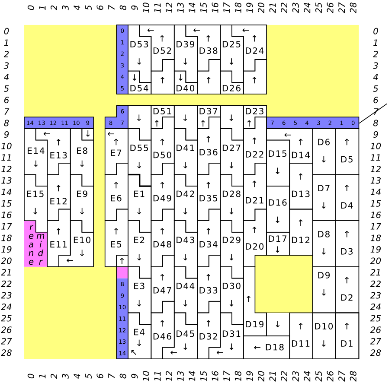
\includegraphics[width=0.9\linewidth]{encoding1}
\caption[encoding]{QR码的编码顺序}
\label{fig:encoding1}
\end{figure}

其中“D”开头的格子表示数据段,“E”开头的格子表示纠错段,浅紫色区域表示格式信息和版本信息。
